\documentclass{article}
\usepackage[utf8]{inputenc}
\usepackage[croatian]{babel}
\usepackage{pgfplots}
\usepackage{hyperref}
\usepackage{booktabs}
\usepackage{amsmath}
\usepackage{amssymb}
\pgfplotsset{compat=1.18}


\begin{document}

\section{Uvod}

Društvene mreže danas obuhvaćaju više od 5,4 milijarde korisnika globalno. Uz stvarne ljude, na njima u velikoj mjeri djeluju botovi. 

Dok \textit{good} botovi obavljaju korisne funkcije (agregacija vijesti, moderatori sadržaja, chatbotovi za podršku), \textit{bad} botovi predstavljaju ozbiljnu kibernetičku i društvenu prijetnju. Oni narušavaju povjerenje u online komunikaciju, manipuliraju javnim mnijenjem i šire dezinformacije. Razvoj alata za detekciju botova je zato ključan jer društvene mreže nagrađuju veliki angažman i gledanost bez obzira na autentičnost. Osim jednostavnih \textit{spam} botova, problem postaju sofisticirani društveni botovi koji oponašaju stvarne osobe.

Osim detekcije botova temeljem broja objava, omjera pratitelja i vjerodostojnosti profila, naš projekt pokušava detektirati bota na temelju same analize teksta i načina pisanja komentara. Zbog veće preciznosti, naš sustav kombinira rad tri različita programera kroz arhitekturu \textbf{ansambla modela} (\textit{Ensemble Learning}).


\section{Matematička analiza i TF-IDF logistička regresija}

\subsection{Dokumentacija podsustava \texttt{tf-logreg}}

Podsustav \texttt{tf-logreg} služi kao brz, lokalno izvediv i objašnjiv osnovni model za detekciju AI-generiranih Reddit komentara. Ulaz u model je isključivo tekst komentara, a izlaz je binarna oznaka \texttt{AI} ili \texttt{HUMAN}. Model ne koristi metapodatke o korisniku, vremenu objave, karmi, povijesti računa ili subredditu. Time je metoda strože ograničena, ali i prikladna za stvarne situacije u kojima je dostupan samo sadržaj komentara.

Mapa \texttt{tf-logreg/} sadrži četiri glavne datoteke. Datoteka \texttt{train.py} trenira model iz CSV datoteke koja mora imati stupce \texttt{comment} i \texttt{label}. Datoteka \texttt{predict.py} učitava spremljeni model i klasificira jedan komentar zadan iz naredbenog retka. Datoteka \texttt{test\_data.py} vrednuje već trenirani model na vanjskom označenom skupu podataka. Datoteka \texttt{reddit\_ai\_detector.joblib} sadrži spremljeni \texttt{scikit-learn} cjevovod, uključujući i pretvorbu teksta u značajke i završni klasifikator.

\paragraph{Ulazni podaci.}
Očekivani format podataka je CSV oblika

\[
\texttt{comment,label},
\]

gdje je \texttt{comment} tekst Reddit komentara, a \texttt{label} oznaka razreda. U implementaciji se uklanjaju retci kojima nedostaje komentar ili oznaka, a oznake se tretiraju kao tekstualne vrijednosti. Prije treniranja provjerava se da skup sadrži barem dva razreda, jer binarna klasifikacija nema smisla ako su svi primjeri iste vrste.

\paragraph{Podjela na skup za učenje i testiranje.}
Skripta \texttt{train.py} koristi \texttt{train\_test\_split} s parametrom \texttt{stratify=y}. Stratifikacija čuva približno isti omjer razreda u skupu za učenje i skupu za testiranje. To je važno jer bi slučajna podjela bez stratifikacije mogla dati testni skup koji nije reprezentativan, posebno ako je jedan razred češći od drugoga.

\paragraph{TF-IDF značajke.}
Komentar se pretvara u numerički vektor pomoću TF-IDF reprezentacije. Za termin $t$ i dokument $d$ težina je

\[
x_{t,d}=\operatorname{tf}(t,d)\cdot \operatorname{idf}(t),
\]

gdje $\operatorname{tf}(t,d)$ mjeri koliko se termin često pojavljuje u komentaru, a $\operatorname{idf}(t)$ smanjuje važnost termina koji su česti u gotovo svim komentarima. Jednostavan oblik IDF faktora je

\[
\operatorname{idf}(t)=\log\frac{N}{1+\operatorname{df}(t)},
\]

pri čemu je $N$ broj dokumenata, a $\operatorname{df}(t)$ broj dokumenata u kojima se termin pojavljuje. Time rijetki, ali informativni izrazi dobivaju veću težinu od vrlo čestih izraza.

U implementaciji se koriste dvije vrste TF-IDF značajki. Prva su riječima temeljene značajke, s unigramima i bigramima, zadane parametrom \texttt{ngram\_range=(1,2)}. One hvataju pojedine riječi i kratke fraze. Druga su znakovne značajke, s nizovima znakova duljine od 3 do 5, zadane parametrom \texttt{ngram\_range=(3,5)}. One hvataju interpunkciju, nastavke riječi, prefikse, tipične obrasce formatiranja i sitne stilističke razlike. Obje se skupine spajaju pomoću \texttt{FeatureUnion}.

\paragraph{Logistička regresija.}
Nakon pretvorbe teksta u vektor $x$, model uči linearnu funkciju

\[
z=w^\top x+b.
\]

Vrijednost $z$ zatim se pretvara u vjerojatnost sigmoidnom funkcijom

\[
P(y=1\mid x)=\sigma(z)=\frac{1}{1+e^{-z}},
\]

gdje $y=1$ označava razred \texttt{AI}. Ako je procijenjena vjerojatnost veća za razred \texttt{AI}, model vraća \texttt{AI}; inače vraća \texttt{HUMAN}. Tijekom treniranja minimizira se binarna unakrsna entropija

\[
\mathcal{L}(w,b)=-\frac{1}{m}\sum_{i=1}^{m}\left[y_i\log(p_i)+(1-y_i)\log(1-p_i)\right],
\]

gdje je $p_i=P(y_i=1\mid x_i)$. U kodu se koristi \texttt{class\_weight="balanced"}, čime se smanjuje rizik da model favorizira većinski razred.

\paragraph{Izlaz i sigurnost predikcije.}
Skripta \texttt{predict.py} koristi metodu \texttt{predict\_proba}, pa izlaz nije samo konačna oznaka, nego i procijenjena vjerojatnost za svaki razred. Ta se vrijednost može tumačiti kao sigurnost modela, ali ne kao dokaz da je komentar stvarno napisao čovjek ili AI. Visoka vjerojatnost znači da je komentar sličan obrascima koje je model naučio iz trening podataka.

\paragraph{Pokretanje.}
Treniranje modela može se pokrenuti naredbom

\[
\texttt{uv run python tf-logreg/train.py --data data/train.csv}.
\]

Vrednovanje spremljenog modela na testnom skupu pokreće se naredbom

\[
\texttt{uv run python tf-logreg/test\_data.py --data data/test.csv}.
\]

Klasifikacija jednog komentara pokreće se naredbom

\[
\texttt{uv run python tf-logreg/predict.py --text "Primjer komentara"}.
\]

Isti spremljeni model koristi i lokalni FastAPI poslužitelj u datoteci \texttt{app.py}, koji izlaže endpoint \texttt{/classify}. Chrome ekstenzija šalje tekst komentara tom lokalnom endpointu i prikazuje oznaku korisniku.

\paragraph{Ograničenja.}
Ovaj podsustav je brz i praktičan, ali ima jasna ograničenja. Budući da koristi samo tekst, ne može prepoznati obrasce ponašanja računa. Budući da uči iz označenog skupa podataka, njegova kvaliteta ovisi o reprezentativnosti tog skupa. Formalno napisani ljudski komentari mogu izgledati kao AI, dok AI komentari s namjernim pogreškama mogu izgledati ljudski. Zbog toga se \texttt{tf-logreg} koristi kao jedan član šireg ansambla, zajedno sa semantičkim SVM-om, perplexity mjerom, sentiment analizom i završnim modelom za spajanje rezultata.

\subsection{Aproksimirani uspon botova}

\begin{figure}[h!]
    \centering
    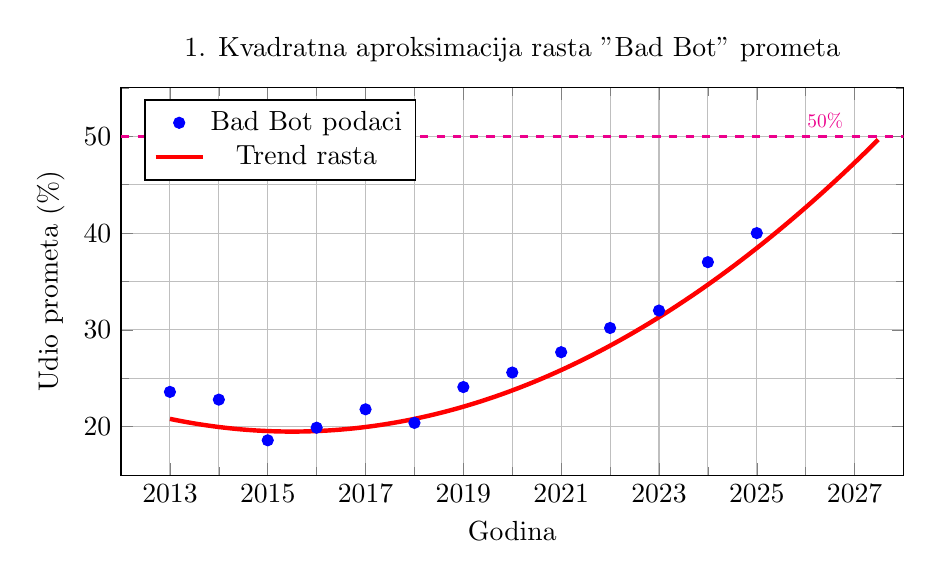
\begin{tikzpicture}
        \begin{axis}[
            title={1. Kvadratna aproksimacija rasta "Bad Bot" prometa},
            xlabel={Godina},
            ylabel={Udio prometa (\%)},
            xmin=2012, xmax=2028, 
            ymin=15, ymax=55,      
            xticklabel style={/pgf/number format/set thousands separator={}},
            xtick={2013, 2015, 2017, 2019, 2021, 2023, 2025, 2027},
            grid=both,
            minor tick num=1,
            legend pos=north west,
            width=0.95\textwidth,
            height=6.5cm,
        ]
            \addplot[blue, only marks, mark=*, mark size=2pt] coordinates {
                (2013, 23.6) (2014, 22.8) (2015, 18.6) (2016, 19.9) 
                (2017, 21.8) (2018, 20.4) (2019, 24.1) (2020, 25.6) 
                (2021, 27.7) (2022, 30.2) (2023, 32.0) (2024, 37.0)
                (2025, 40.0) 
            };
            \addlegendentry{Bad Bot podaci}

            \addplot[red, ultra thick, domain=2013:2027.5, samples=100] {0.21*(x-2015.5)^2 + 19.5}; 
            \addlegendentry{Trend rasta}
            \draw[magenta, dashed, line width=1pt] (axis cs:2012,50) -- (axis cs:2028,50) node[pos=0.9, above, scale=0.7]{50\%};
        \end{axis}
    \end{tikzpicture}
\end{figure}

\begin{figure}[h!]
    \centering
    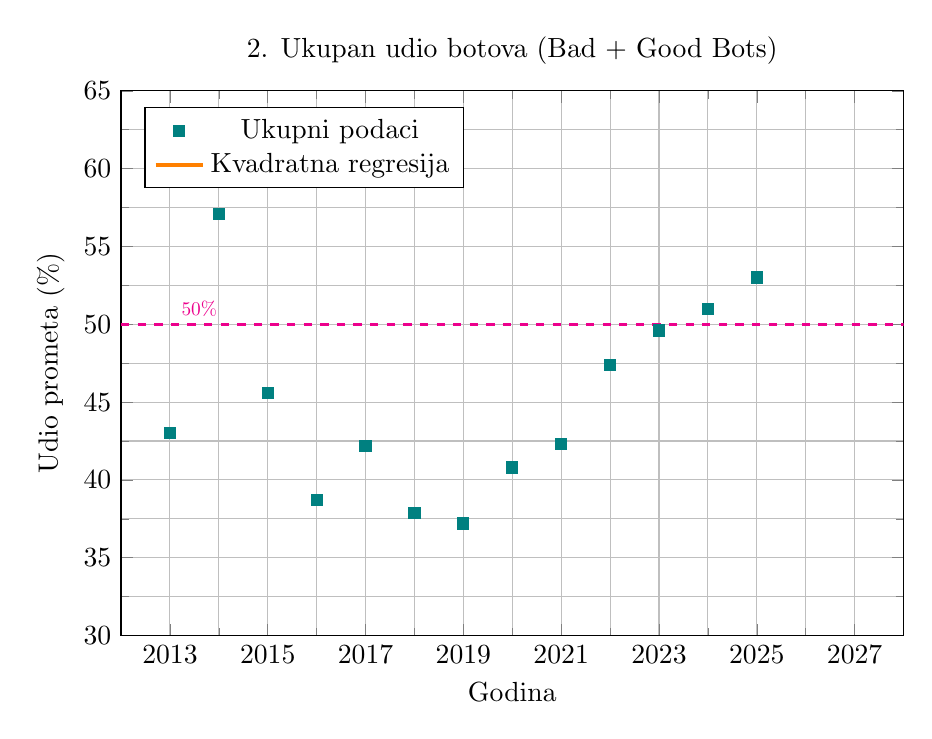
\begin{tikzpicture}
        \begin{axis}[
            title={2. Ukupan udio botova (Bad + Good Bots)},
            xlabel={Godina},
            ylabel={Udio prometa (\%)},
            xmin=2012, xmax=2028, 
            ymin=30, ymax=65,      
            xticklabel style={/pgf/number format/set thousands separator={}},
            xtick={2013, 2015, 2017, 2019, 2021, 2023, 2025, 2027},
            grid=both,
            minor tick num=1,
            legend pos=north west,
            width=0.95\textwidth,
            height=8.5cm,
        ]
            \addplot[teal, only marks, mark=square*, mark size=2pt] coordinates {
                (2013, 43.0) (2014, 57.1) (2015, 45.6) (2016, 38.7) 
                (2017, 42.2) (2018, 37.9) (2019, 37.2) (2020, 40.8) 
                (2021, 42.3) (2022, 47.4) (2023, 49.6) (2024, 51.0)
                (2025, 53.0)
            };
            \addlegendentry{Ukupni podaci}

            \addplot[orange, ultra thick, domain=2013:2028, samples=100] {0.15814*x^2 - 639.186*x + 645164}; 
            \addlegendentry{Kvadratna regresija}
            \draw[magenta, dashed, line width=1pt] (axis cs:2012,50) -- (axis cs:2028,50) node[pos=0.1, above, scale=0.7]{50\%};
        \end{axis}
    \end{tikzpicture}
    \caption{\footnotesize \textit{https://www.statista.com/statistics/1264226/human-and-bot-web-traffic-share/}}
\end{figure}

\subsection*{Kratka interpretacija anomalije iz 2014.}
Nagli skok bot prometa u 2014. godini uzrokovan je masovnim sigurnosnim skeniranjima (Heartbleed, Shellshock) i intenzivnim indeksiranjem web stranica. Naknadni pad rezultat je uvođenja boljih sustava zaštite (poput Cloudflarea) i optimizacije rada tražilica, prije novog vala rasta potaknutog modernim AI alatima.

\begin{table}[h!]
\centering
\caption{Ključne metrike internetskog prometa i sigurnosti (Izvještaj 2026.)}
\vspace{2mm}
\begin{tabular}{@{}llc@{}}
\toprule
\textbf{Kategorija} & \textbf{Metrika} & \textbf{Vrijednost} \\ \midrule
\textbf{Promet} & Udio botova u ukupnom prometu & 53\% \\
 & Udio ljudskog prometa & 47\% \\
\textbf{Sigurnost} & Udio "loših" (bad) botova & 40\% \\
 & Godišnji porast AI bot napada & 12.5x \\
\textbf{Infrastruktura} & Bot napadi na API-je & 27\% \\
 & Bot napadi na poslovnu logiku & 21\% \\
\textbf{Metode} & Botovi koji koriste Chrome za prikrivanje & 41\% \\
\textbf{Industrija} & Napadi na financijske usluge & 24\% \\
 & Preuzimanje računa (ATO) u financijama & 46\% \\ \bottomrule
\end{tabular}
\begin{flushleft}
\footnotesize \textit{Izvor: Analiza Bad Bot Report 2026 (Thales/Imperva). https://www.imperva.com/resources/resource-library/reports/2026-bad-bot-report/}
\end{flushleft}
\end{table}
\subsection{Semantički SVM kao podsustav klasifikacije}

\paragraph{Motivacija.}
Uvođenje ovoga podsustava polazi od pretpostavke da se znatan dio AI-generiranih komentara ne razlikuje samo po stilu pisanja, nego i po semantičkoj namjeni. Takvi su komentari često oblikovani tako da pojačaju angažman: izazovu ljutnju, prodube političku ili ideološku podjelu, zaoštre raspravu ili potaknu niz daljnjih reakcija. Zbog toga je razumno očekivati da se u prostoru značenja pojavljuju obrasci koji nisu slučajni i koje je moguće geometrijski razdvajati. Ne tvrdi se da svaki AI komentar nužno ima takvu funkciju, nego da je taj signal dovoljno čest da ga vrijedi zasebno modelirati. U tom smislu ovaj podsustav ne traži samo pojedine riječi, nego pokušava razdvojiti komentare prema njihovoj semantičkoj ulozi.

Semantički SVM pridružuje komentaru $t$ vrijednost

\[
p_{\mathrm{sem}}(t) \approx P(y=1\mid t),
\]

pri čemu $y=1$ označava razred \texttt{AI}, a $y=0$ razred \texttt{HUMAN}. Ta se vrijednost dalje koristi kao jedan od triju ulaza završnog modela.

\paragraph{Vektorski prikaz i predobrada.}
Tekst se najprije prevodi u semantički vektorski prikaz $x$, zatim normira

\[
\hat{x}=\frac{x}{\|x\|_2},
\]

a potom standardizira po koordinatama

\[
z_j=\frac{\hat{x}_j-\mu_j}{\sigma_j}.
\]

L2-normiranje uklanja razlike u duljini vektora, dok standardizacija usklađuje mjerila pojedinih koordinata prije učenja linearnog razdjelnika.

Takav je slijed važan jer SVM ne radi nad rečenicama kao nizovima znakova, nego nad točkama u prostoru $\mathbb{R}^d$. Ugrađivački model već je prije toga proveo nelinearno semantičko preslikavanje teksta u vektor, pa klasifikator više ne razdvaja "riječi", nego geometrijske položaje komentara u dobivenom prostoru.

\paragraph{Zašto je linearan razdjelnik ovdje prirodan izbor.}
Nakon ugradnje tekst više nije prikazan u izvornom prostoru, nego u prostoru semantičkih značajki. Složeniji, nelinearni dio posla već je obavio model za vektorske prikaze. Zbog toga linearan SVM u tom novom prostoru često daje vrlo dobar kompromis između interpretabilnosti, brzine i točnosti. Drugim riječima, nelinearnost je sadržana u prikazu, a ne u samoj završnoj klasifikacijskoj funkciji.

\paragraph{Odlučna funkcija i geometrija margine.}
Nad vektorom $z$ uči se linearna odlučna funkcija

\[
f(z)=w^\top z+b.
\]

Granica razdvajanja zadana je jednadžbom $w^\top z+b=0$, a rubovi margine jednadžbama $w^\top z+b=\pm 1$. Budući da širina margine iznosi

\[
\frac{2}{\|w\|_2},
\]

minimizacija člana $\frac{1}{2}\|w\|_2^2$ ekvivalentna je maksimizaciji margine. Model, dakle, traži što širi pojas razdvajanja dvaju razreda.

To se može pokazati izravno. Neka su $z_+$ i $z_-$ točke na dvama rubovima margine, pa vrijedi

\[
w^\top z_+ + b = 1,
\qquad
w^\top z_- + b = -1.
\]

Oduzimanjem dobivamo

\[
w^\top (z_+ - z_-) = 2.
\]

Najkraća udaljenost dviju paralelnih hiperravnina mjeri se u smjeru njihova normale $w$, pa je $z_+ - z_- = \lambda w$ za neki skalar $\lambda$. Uvrštavanjem slijedi

\[
w^\top(\lambda w)=\lambda\|w\|_2^2=2,
\qquad
\lambda=\frac{2}{\|w\|_2^2}.
\]

Stoga je udaljenost između rubova margine

\[
\|z_+-z_-\|_2 = |\lambda|\,\|w\|_2 = \frac{2}{\|w\|_2}.
\]

Upravo zato minimizacija norme vektora $w$ znači širenje margine.

\paragraph{Optimizacija meke margine.}
Za oznake $\tilde y_i\in\{-1,+1\}$ rješava se problem

\[
\min_{w,b,\xi}\;\frac{1}{2}\|w\|_2^2 + C\sum_{i=1}^n \xi_i
\]

uz ograničenja

\[
\tilde y_i(w^\top z_i+b)\ge 1-\xi_i,
\qquad
\xi_i\ge 0.
\]

Polazište je tvrda margina, gdje bi se zahtijevalo $\tilde y_i(w^\top z_i+b)\ge 1$ za svaki primjer. Budući da stvarni tekstualni podaci nisu savršeno razdvojivi, uvodi se meka margina preko varijabli $\xi_i$.

Izraz $\tilde y_i(w^\top z_i+b)$ objedinjuje oba razreda u jednom uvjetu: pozitivan je kada je primjer na ispravnoj strani granice, a negativan kada je pogrešno razvrstan. Time jedno ograničenje istodobno pokriva i AI i HUMAN razred. Varijabla $\xi_i$ mjeri povredu idealne margine, pa vrijedi: $\xi_i=0$ za ispravno razvrstane primjere izvan margine, $0<\xi_i<1$ za primjere unutar margine, $\xi_i=1$ za primjere točno na granici odluke, a $\xi_i>1$ za pogrešno razvrstane primjere. Parametar $C$ određuje odnos između širine margine i kazne za pogreške: veći $C$ snažnije kažnjava povrede, a manji $C$ dopušta pravilniju, ali fleksibilniju granicu.

Isti se problem može zapisati i preko hinge-gubitka

\[
\ell_{\mathrm{hinge}}(\tilde y,f(z)) = \max\{0,1-\tilde y f(z)\},
\]

pa optimizacijska zadaća poprima oblik

\[
\min_{w,b}\;\frac{1}{2}\|w\|_2^2 + C\sum_{i=1}^n \max\{0,1-\tilde y_i(w^\top z_i+b)\}.
\]

Taj zapis jasno pokazuje zašto primjeri daleko od granice ne pridonose gubitku, dok primjeri unutar margine i pogrešno razvrstani primjeri nose kaznu.

\paragraph{Dualna formulacija i računalna provedba.}
U dualnoj formulaciji vrijedi

\[
w=\sum_{i=1}^n \alpha_i \tilde y_i z_i,
\]

pa na granicu razdvajanja bitno utječu samo primjeri s $\alpha_i>0$, odnosno potporni vektori. Oni su geometrijski oni primjeri koji ``nose'' razdvajanje: leže na rubu margine ili narušavaju njezine uvjete. Ta formulacija objašnjava zašto o svim primjerima ne ovisi završna granica jednako.

U klasičnom kernel-SVM pristupu dualni se problem često rješava metodama poput SMO postupka, jer je tada prirodno raditi s unutarnjim produktima među primjerima. U stvarnoj provedbi ovoga podsustava to nije slučaj: ovdje se koristi \texttt{LinearSVC} nad standardiziranim semantičkim prikazima. Zato je dualna slika važna za matematičko razumijevanje modela, ali nije doslovan opis numeričkog postupka koji se izvršava u kodu.

\paragraph{Vjerojatnosna kalibracija.}
SVM izravno daje potpisanu vrijednost odlučne funkcije

\[
s=f(z)=w^\top z+b,
\]

a ne vjerojatnost. Zbog toga se primjenjuje Plattova kalibracija

\[
P(y=1\mid s)\approx \frac{1}{1+\exp(As+B)}.
\]

To ima jasnu interpretaciju: velike pozitivne vrijednosti $s$ trebaju odgovarati vjerojatnostima bliskima $1$, velike negativne vrijednosti vjerojatnostima bliskima $0$, a prijelaz oko granice odvija se glatko, bez skokova. Parametri $A$ i $B$ određuju nagib i položaj te sigmoidne preslikbe.

Parametri $A$ i $B$ uče se isključivo na skupu za učenje, i to trostrukom unakrsnom kalibracijom: u svakom presjeku bazni \texttt{LinearSVC} trenira se na dvjema trećinama podataka, na preostaloj trećini računaju se vrijednosti odlučne funkcije, a na njima se zatim prilagođava sigmoidna funkcija. Time se izbjegava kalibriranje na istim vrijednostima na kojima je razdjelnik upravo naučen. Završna procjena dobiva se kao prosjek triju kalibriranih vjerojatnosti. Razvojni skup pritom ostaje odvojen i služi samo za vrednovanje.

\paragraph{Izlaz podsustava.}
Za pojedini komentar podsustav vraća kalibriranu vjerojatnost $p_{\mathrm{sem}}(t)$. Kad bi se koristio samostalno, binarna bi odluka mogla biti zadana pravilom

\[
\hat y = \mathbf{1}\{p_{\mathrm{sem}}(t)\ge 0.5\}.
\]

U ovom radu to nije središnje, jer završni model koristi samu vjerojatnost, a ne unaprijed zadani prag.

\paragraph{Rezultati na razvojnom skupu.}
Na punom skupu za učenje, uz unaprijed izračunate semantičke vektorske prikaze, dobivene su vrijednosti točnosti $0.90948$, preciznosti $0.90341$, odziva $0.91283$, mjere $F_1=0.90810$ i pokazatelja $\mathrm{ROC\ AUC}=0.96885$. Konfuzijska matrica na razvojnom skupu iznosi

\[
\begin{array}{c|cc}
 & \hat y=0 & \hat y=1 \\
\hline
y=0 & 19549 & 2022 \\
y=1 & 1806 & 18912
\end{array}
\]

što pokazuje da podsustav dobro razdvaja razrede i daje pouzdanu procjenu vjerojatnosti AI razreda.

\paragraph{Mogućnost jednostavnog poboljšanja.}
Najizravnije poboljšanje ovoga podsustava jest zamjena sadašnjeg modela za izradu semantičkih vektorskih prikaza snažnijim modelom, uz zadržavanje iste SVM i kalibracijske sheme. Drugim riječima, ne mijenja se klasifikator, nego kvaliteta prikaza na kojem on radi. U sadašnjoj izvedbi korišten je \texttt{all-MiniLM-L6-v2} zbog brzine, dok bi prirodan sljedeći korak bio \texttt{BAAI/bge-small-en-v1.5}, a uz više računalnih resursa i veći modeli iste namjene. Takva je izmjena tehnički jednostavna, ali računski skuplja, jer najveći dio vremena i dalje otpada na izradu semantičkih vektorskih prikaza.
\end{document}
